

\documentclass[a4paper]{article}

\usepackage[english]{babel}
\usepackage[utf8]{inputenc}
\usepackage{amsmath}
\usepackage{graphicx}
\usepackage{fancyref}
\usepackage{amsmath}
\usepackage{listings}
\usepackage{url}
\usepackage{float}
\usepackage{amssymb}
\usepackage{rotating}
\usepackage{multirow}
\usepackage[toc,page]{appendix}

\usepackage{tikz}
\usepackage[ruled,linesnumbered,vlined]{algorithm2e}

\usepackage{verbatim}

\newcommand{\norm}[1]{\left\lVert#1\right\rVert}
\newcommand{\argmin}{\arg\!\min}


\title{Adversarial training on neural networks.}

\author{Marc Moreaux}

\date{\today}

\begin{document}
\maketitle



\section{Introduction} 
\label{sec:introduction}
	
	This machine learning master thesis is about neural networks (section \ref{sec:neural_networks}). 


	\subsection{Motivation}
		At the very beginning of this thesis, there is me, the writer. I wanted, from the very first day, to work on neural-networks and more specifically on deep-learning. I wanted so, because deep-learning has become in the last decade the most efficient algorithm at classifying images. 
		I was then searching for a topic. I discovered the work made by Ian J. Goodfellow, Jonathon Shlens and Christian Szegedy. In their publication named "Explaining and Harnessing Adversarial Examples"\cite{goodfellow2014explaining} they motivate that adversarial learning could improve the accuracy of some given neural-networks. After contacting one of the authors of this publication, it appeared that it would be a good contribution to validate their observations on other datasets, since most of their test are based on the MNIST dataset\cite{lecun-mnist}. Therefore, the following thesis is about further validating the proposed adversarial-learning method described in \cite{goodfellow2014explaining} with different datasets.

	\subsection{Methodology}
		We are therefore going to investigate on how is adversarial-learning performing with shallow-neural-networks on different datasets. On the same time, we are going to investigate on the reasons underlining this performances. To do so, we will first re-implement the proposed solution of \cite{goodfellow2014explaining} in such a way that we isolate adversarial-learning from other techniques used in the paper. At this point we will emphasize the benefits of adversarial-learning. 

		We will then move to another dataset similar to the first one, there will also be 10 different classes of images to classify. That dataset will be the CIFAR10\cite{CIFAR10_BITCHES}. Again, some knowledge will be acquired from this experience. Finally, we will test the adversarial-learning on a dataset of other nature. The one we would try is a phoneme dataset: the TIMIT dataset\cite{maybe...}. The results obtained from this dataset will further validate the technique as useful for classification in the context of shallow-neural-network.

	\subsection{Expected outcome}
		In their paper, Ian J. Goodfellow, Jonathon Shlens and Christian Szegedy, described their technique to able to ??? 
		=> How adversarial learning best separate the classes.
		With this adversarial-learning technique we expect to have a network able to emphasize the differences the classes. We expect the network to learn the differences between classes more than just the pattern of a class.


	\subsection{Adversarial-learning}
		Until now, we've been teasing adversarial-learning without explaining what it is about. Lets start off with mentioning what an adversarial sample to a classifier would be. Imagine you have full knowledge of a given classifier. Starting from there, you can create samples to this classifier that are going to give some predictions. Knowing how does the classifier behaves, you can creates samples leading your classifier to some mistakes. This are adversarial samples. In machine learning, adversarial-learning is about creating a classifier resisting to adversarial samples.

		In the publication that interest us\cite{goodfellow2014explaining}, the authors noticed that twisting each pixels of the input images by some very specific values (the adversarial values), an accurate classifier could be easily fooled. Lets detail : Consider you have a classifier able to recognize the MNIST dataset and this classifier makes 10 errors when guessing the classes of 200 samples. Now, if you modify each pixels of these 200 samples by a little value, the classifier makes 180 errors. You've fooled your classifier. 

		The adversarial-learning algorithm we use, is going to embed some properties letting the classifier resist to some adversarial samples. More specifically, we are going to train our classifier on adversarial samples that could have been used to fool our classifier.



	\subsection{Setting-up an example}
		To understand our adversarial training we will use a simple neural network composed by two sigmoid neurons (see section \ref{sec:Artificial_neurons}). The network aims a recognizing a columns and a dot in a three by one pixels image. This network is sketched on \fref{fig:2N_NN}. Considering a white pixel has value $1$ and a dark pixel has value $0$, a column could be represented by a vector $x^1 = [1,0,1]$ and a dot could be by $x^2 = [0,0,1]$. We consider the column to be the output $y^i = 0$ and the dot to be the output $y^i = 1$
		To predict a sensible value, a two-sigmoid network could use the weights and biases :
		$$ W = \left( \begin{matrix} 1 & -1 \\ -1 & -1 \\ 1 & 1 \end{matrix} \right) ; b = \left( \begin{matrix} -1.5 & 0.5 \end{matrix} \right)$$
		
		\vskip 1em
		\textbf{signal propagation: } The input signal $x^i$ propagates through the network resulting in a prediction vector $p^i = \sigma(W^Tx + b)$. To know how right or wrong is this prediction vector, we would use a cost function like the negative log-likelihood:
		$$ C^i = y^i \ln(p^i) + (1-y^i)\ln(1-p^i) $$
		Propagating $x^1$ and $x^2$, we get that $p^1 = [\sigma(.5), \sigma(-.5)]$ and $p^2 = [\sigma(-.5), \sigma(.5)]$

		\begin{figure}
			\centering
			\def\layersep{1.5cm}	
			\begin{tikzpicture}[shorten >=1pt,->,draw=black!50, node distance=\layersep]
			    \tikzstyle{every pin edge}=[<-,shorten <=1pt]
			    \tikzstyle{pixel} = [rectangle, fill=black!10,minimum size=17pt,inner sep=0pt]
			    \tikzstyle{neuron}=[circle,fill=black!25,minimum size=17pt,inner sep=0pt]
			    \tikzstyle{annot} = [text width=5em, text centered]
			    \tikzstyle{annot2} = [text width=18em, text centered]
				\tikzstyle{accolade} = [rectangle, text centered, minimum size=17pt]
			    
			    %%% DRAW THE NODES
			    \foreach \name / \y in {1,2,3}
			        \node[pixel] (I-\name) at (0,-\y) {$x^i_\y$};
			    \node[] (I-4) at (\layersep/2,-3.5) {$1$};
			    \foreach \name / \y in {1,2}
					\node[neuron] (O-\y) at (\layersep*2,-\y-0.5) {$\sigma(z_\y)$};
				\foreach \name / \y in {1,2}	
					\node[] (C-\y) at (\layersep*3,-\y-0.5) {$p^i_\y$};

			    %%% DRAW THE PATHS
			    \foreach \source in {1,...,4}
			        \foreach \dest in {1,2}
			            \path (I-\source) edge (O-\dest);
			    \foreach \y in {1,2}
			        \path (O-\y) edge (C-\y);

			    %%% ANOTATE
			    \node[accolade] at (\layersep*3+1em,-2) { \Huge\} };
			    \node[annot2] at (\layersep*3+10.5em,-2) (cost) {$C^i = \sum_k y^i_k \ln(p^i_k) + (1-y^i_k)\ln(1-p^i_k) $};

			    \node[annot,above of=I-1, node distance=1cm] (iv) {Pixels};
			    \node[annot,above of=O-1, node distance=1cm] (iv) {Neurons};
			    \node[annot,above of=cost, node distance=1cm] (iv) {Cost};

			\end{tikzpicture}
			\label{fig:2N_NN}
			\caption{Two neurons neural network}
		\end{figure}


	\subsection{Adversarial learning}
		Imagine you are allowed to modify each pixels of our image by a value $\epsilon$. Intuitively, if you want to improve the recognition, you would increase the contrast in the picture and insist on the dots where the aught to be. On the other hand, if you want to confuse the recognition, you would lower the contrast and add color where there shouldn't be.

		These properties are the ones we aught to enforce with our adversarial learning. For an epsilon small enough, we subtract to $x^i$ $\epsilon$ times the sign of the derivative with respect to $x^i$ of the Cost $C^i$.
		$$ x^{i_{\text{adv}}} \leftarrow x^i - \epsilon \text{ sign}(\nabla_{x^i} C^i) $$
		Therefore the input $x^i$ is modified such that ?? TODO: HERE IS THE THING ??

		\vskip 1em
		\textbf{In our example. } We apply the adversarial learning to our example. First we compute the derivative of the Cost with respect to $x^i$. (The mathematics behind this derivative is detailed on the appendix \ref{sec:2N_NN_cost})
		$$	\frac{\delta C^i}{\delta x^i} = W \cdot \left( y^i -p^i \right) $$
		Then we subtract the sign of this derivative to the actual input $x^i$
		\begin{equation}
			\begin{split}
				x^{1_{\text{adv}}} &\leftarrow x^1 - \epsilon \text{ sign}(\nabla_{x^1} C(W,b,x^1)) \\
				x^{1_{\text{adv}}} &\leftarrow x^1 - \epsilon \text{ sign}( W \cdot ( y^i -p^i) )
			\end{split}
		\end{equation}
		\begin{equation}
			x^1 = \left( \begin{matrix} 1 \\ 0 \\ 1 \end{matrix} \right) ;
			x^{1_{\text{adv}}} = \left( \begin{matrix} .7 \\ 0 \\ 1 \end{matrix} \right) ;
			x^2 = \left( \begin{matrix} 0 \\ 0 \\ 1 \end{matrix} \right) ;
			x^{2_{\text{adv}}} = \left( \begin{matrix} .3 \\ 0 \\ 1 \end{matrix} \right) ;
		\end{equation}
		


		Once we have these derivatives, the worst modification we can make to sample $x^i$ is by following this derivative. 
		

	\subsection{Dataset}
		The first dataset we will be using is the MNIST\ref{??} dataset. This dataset is composed by 60k gray scale images. Each of them represent a hand written digit (6k of each). 







		

\section{Neural-Networks}
\label{sec:neural_networks}

	In this section we will see how neural-network manage to solve classification tasks. As a reminder, a classification problem aims at identifying the sub-populations of a set belonging to a class. More specifically : if we are given a set of inputs $X$ and outputs $Y$. where $x^i$ denotes a sample from the set $X$ and $y^i$ its class. Then, the aim of classification is to predict the class a new sample given the knowledge based on the $x^i$'s.

	Artificial neural-networks are a family of statistical learning algorithms. They are inspired from the human brain structure : nowadays, we believe the brain has a network of neurons triggering signals over its dendrite and propagated to other neurons through a synapse interface. Network of artificial neurons mimics these properties.

	In this section, we will first introduce what are the artificial neurons and how do we aggregate them to make neural-networks. After we've seen this, we will see how to train these networks: what is a cost and how do we reduce the error made by these networks.


	\subsection{Artificial neuron and Perceptron}
	\label{sec:Artificial_neurons}
		First, the neurons. The first neuron we mention here is the \textbf{Perceptron}. It was described by Rosenblatt in 1958 \cite{rosenblatt1958perceptron} and was one of the first artificial neuron introduced in the literature. This neuron takes as an input multiple binary values to which it apply weights. Once multiplied, these \textit{weighted inputs} are summed-up. If the sum is lower than zero, the neuron outputs zero. Otherwise, the neuron outputs one. A schema of an artificial neuron is given on \Fref{fig:perceptron}.

		Formally: given an input vector $x$ of size $m$ where $x_i$ is the $i$th element of $x$, the Perceptron defines a weight vector $w$ with same shape as the input vector $x$ and a bias term $b$. Then its transfer function is :

		$$ \text{Perceptron}(x) = \begin{cases}1 & \text{if } \sum_{j=0}^m (w_j \times x_j) + b > 0\\0 & \text{otherwise}\end{cases} $$

		In a vector notation this becomes 

		$$ \text{Perceptron}(x) = \begin{cases}1 & \text{if } w^T \cdot x +b > 0\\0 & \text{otherwise}\end{cases} $$

		\begin{figure}
			\centering
			\def\layersep{1.5cm}
			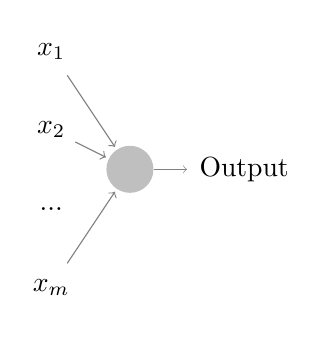
\begin{tikzpicture}[shorten >=1pt,->,draw=black!50, node distance=\layersep]
				\tikzstyle{tata}=[,minimum size=17pt,inner sep=0pt]
			    \tikzstyle{neuron}=[circle,fill=black!25,minimum size=17pt,inner sep=0pt]
			    \tikzstyle{output neuron}=[neuron, fill=red!50];

			    % Input neurons
			    \node[tata] (x1) at (0,-1 cm) {$x_1$};
			    \node[tata] (x2) at (0,-2 cm) {$x_2$};
			    \node[tata] (x3) at (0,-3 cm) {...};
			    \node[tata] (x4) at (0,-4 cm) {$x_m$};
			    
			    % Draw the output layer node
			    \node[neuron,pin={[pin edge={->}]right:Output}] (O) at (\layersep,-2.5) {};

			    % Connect every node in the hidden layer with the output layer
			    \path (x1) edge (O);
			    \path (x2) edge (O);
			    \path (x4) edge (O);

			\end{tikzpicture}
			\label{fig:perceptron}
			\caption{Model of an artificial neuron}
		\end{figure}

		Nowadays we use other types of neurons. As the Perceptron, these neurons consider a weighted sum of their inputs plus a bias term. Now, their activation function is different and their outputs are real valued. We present two of the well known neurons:
		\begin{itemize}
			\item The \textbf{sigmoid neuron} is defined by a smooth threshold function :
			$$ \sigma(x) = \frac{1}{1 + e^{-x}} $$
			\item The \textbf{Regression Logistic Unit} (ReLU) is a neuron which activation function is equal to zero for any negative inputs and equal to its input otherwise.
			$$ \text{ReLU}(x) = \begin{cases} ?? & \text{if } w \cdot x + b > 0 \\0 & \text{otherwise}\end{cases} $$
		\end{itemize}


	\subsection{Neural-network}
		Now that we have neurons, we need a network of them to compose an architecture similar to the brain. The networks we are going to work with are called \textbf{feed-forward} neural-networks. They are the most common ones in the literature. \Fref{fig:feed_forward} is a representation of a two-hidden-layer feed-forward neural-network. As you can see, this model consist of groups of neurons. We denote as layer the group of neurons belonging to the same deepness in the model. Therefore, all the neurons visible on the left in our model, compose the first layer of neurons. It's the input layer. The following layers are called the hidden layers and the last one is the output layer. Some variations exists of this definition, for instance, some outputs of the model might be placed at the same level as some hidden layer.

		Our simple example is also a feed-forward neural-network. It has an input layer fully connected to a hidden layer, which is also fully connected to the output layer. As drawn on the schema with the directions of the arrows, the signal propagates from left to right, from the inputs to the outputs. Because of these two reasons (layers fully connected and single direction signal propagation) our simple example is a feed-forward neural-network.		

		\begin{figure}
			\centering
			\def\layersep{1.5cm}
			\begin{tikzpicture}[shorten >=1pt,->,draw=black!50, node distance=\layersep]
			    \tikzstyle{every pin edge}=[<-,shorten <=1pt]
			    \tikzstyle{neuron}=[circle,fill=black!25,minimum size=17pt,inner sep=0pt]
			    \tikzstyle{annot} = [text width=4em, text centered]


			    %%%%%%%%%%%%%%%%%%%%%%%%%%%%%%%%%%%%%%%%%%%% 
			    %%% DRAW THE NODES
			    %%%%%%%%%%%%%%%%%%%%%%%%%%%%%%%%%%%%%%%%%%%%
			    \foreach \name / \y in {1,...,4}
			        \node[] (I-\name) at (0,-\y) {$x_{i\y}$};

			    \foreach \name / \y in {1,...,5}
			        \path[yshift=0.5cm] node[neuron] (H1-\name) at (\layersep,-\y cm) {};

				\foreach \name / \y in {1,...,7}
			        \path[yshift=1.5cm] node[neuron] (H2-\name) at (\layersep*2,-\y cm) {};   

		       	
			    \node[neuron,pin={[pin edge={->}]right:$p_{i1}$}, right of=H2-3] (O-1) {};
			    \node[neuron,pin={[pin edge={->}]right:$p_{i2}$}, right of=H2-5] (O-2) {};

			    %%%%%%%%%%%%%%%%%%%%%%%%%%%%%%%%%%%%%%%%%%%% 
			    %%% DRAW THE PATHS
			    %%%%%%%%%%%%%%%%%%%%%%%%%%%%%%%%%%%%%%%%%%%%
			    \foreach \source in {1,...,4}
			        \foreach \dest in {1,...,5}
			            \path (I-\source) edge (H1-\dest);

			    \foreach \source in {1,...,5}
			        \foreach \dest in {1,...,7}
			            \path (H1-\source) edge (H2-\dest);

			    \foreach \source in {1,...,7}
			    	\foreach \dest in {1,...,2}
				        \path (H2-\source) edge (O-\dest);

			    % Annotate the layers
			    \node[annot,above of=H2-1, node distance=1cm] (hl) {Hidden layer 2};
			    \node[annot,left of=hl] (hl1) {Hidden layer 1};
			    \node[annot,left of=hl1] {Input layer};
			    \node[annot,right of=hl] {Output layer};
			\end{tikzpicture}
			\label{fig:feed_forward}
			\caption{Feed-forward neural-network with two hidden layers}
		\end{figure}


		It's good to mention that other types of network exits such as the \textbf{recurrent networks}. In these networks, there is directed cycles on the graph which means that a neuron can depends on its own output. This model is considered to be closer to the brain structure but the challenge on training these models isn't state of the art. We won't work on these models.

		\textbf{Symmetrically connected} networks is an other types of network, they are called the "Boltzmann machines". They are symmetrical in the sense that connections between neurons exists in the two directions and the weight on this connections is the same in both directions. Here again, we won't work on these models.


	\subsection{Forward propagation}
		

	

	\subsection{Cost function}
		Once we have build our model, we consider a cost function, also called "loss function". This cost function define how good is the model considering an evaluation criterion. In the case of classification, we want to evaluate how good the prediction is doing towards the true output.
		The most famous cost functions in neural-network classification are the squared error and the cross entropy (also called the "negative log-likelihood"). They are defined as follows for a given sample $i$ and output $j$.
		\begin{itemize}
			\item Squared error : $$ l(p_{ij},y_{ij}) = \norm{y_{ij} - p_{ij}}_2^2 $$
			\item Cross entropy : $$ l(p_{ij},y_{ij}) = -\ln(p_{ij})_{y_{ij}}  ??? $$ 
		\end{itemize}

		Lets take an example. Consider the model presented on \fref{fig:feed_forward}. To this model, we input $x_i$ and propagate the signal until the last layer. This last layer gives us the prediction $p_i = [0.9,0.15]$. Given with $x_i$ we had its true prediction $y_i = [1,0]$. We have everything to compute the two loss functions described earlier : 
		\begin{itemize}
			\item Squared error : $$ l(p_{ij},y_{ij}) =  .1^2 + .15^2 $$
			\item Cross entropy : $$ l(p_{ij},y_{ij}) = -\ln(.1)  $$
		\end{itemize}


	\subsection{Back-propagation}
		Back propagation is the 


		\vspace{1em}
		\textbf{Notation : }\\


	\subsection{Gradient descent}

	\section{Multi-layer neural-network}
		The softmax network we've been previoulsy working with is a single-layer  neural-network, composed by softmax units (or softmax neurons). We are now going to work on a network containing more layers. Instead of forwarding our input data $X$ into the softmax units, we will input them into Rectified Linear Units (ReLU).

		\subsection{Rectifiect Linear Units}
		A ReLU is similar to a perceptron but it has a different transfert function. As the perceptron, it has many inputs an one output. The output is a function of the sum of the weighted inputs. This function is defined as :
		$$ h_t(x) =  $$
		All together, the ReLU outputs :
		$$ \text{ReLU}(X) =  (W^Tx_i) $$

		\subsection{Defining the multi-layer net}
		The Multi-layer neural-network we first study has two layers of composed by 500 ReLU neuron each and an output layer of softmax units. 
% 
\section{Softmax} 
\label{sec:softmax}

	We now study the softmax network. Softmax network is a generalization of logistic regression with a sigmoid transfer function. 
	The softmax network, or better said, the softmax layer, outputs a vector summing to one. 

	Here also we consider $x_i \in \mathbb{R}^m$, the input samples from the set $X$ of size $n$ and $y_i$, the output samples from the set $Y$ of size $n$. The output samples correspond in an integer representing the class of the input. We consider there is $k$ possible classes.

	Considering a softmax layer of size $K$ and with $L$ inputs, the softmax function for a neuron $x$ of the layer is defined as follows :
	$$ \text{softmax}(z_{x}) = \sigma(z_{x}) = \frac{e^{z_{x}}}{\sum_{k\in K} e^{z_k}} $$
	The division by the sum of exponentials permits to have the layer summing up to one. For this reason, we can consider the softmax layer to be a normalized output (throughout the layer) of each of the exponential of the $K$ inputs. 

	On the network visible on \fref{fig:softmax}, the signal propagates as follows : First, the input $x_i$ is multiplied with a weight $w_k$, which result in $z_k$, then $\sigma{z_k}$ is computed. 

	\subsection{Softmax derivatives}
		To be able to apply the gradient descent we compute the derivatives of the softmax. Two cases have to be considered. 
		\begin{itemize}
			\item When we derive $\sigma(z_l)$ with respect to $z_l$.
			\begin{equation} \label{eq:grad_sima_zk1}
				\begin{split}
					\frac{\partial \sigma(z_l)}{\partial z_l} 
					&= \frac{ e^{z_l} \sum_{k} e^{z_k} - e^{z_l} e^{z_l}}{ (\sum_{k} e^{z_k})^2 } \\
					&= \frac{ e^{z_l} \sum_{k} e^{z_k} }{ (\sum_{k} e^{z_k})^2 } - \frac{ (e^{z_l})^2 }{ (\sum_{k} e^{z_k})^2 }\\
					&= \sigma(z_l) - \sigma(z_l)^2 \\
					&= \sigma(z_l)(1-\sigma(z_l))
				\end{split}
			\end{equation}

			\item When we derive $\sigma(z_l)$ with respect to any of the other $z_{k}$ inputs ($k != l$).
			\begin{equation} \label{eq:grad_sima_zk}
				\begin{split}
					\frac{\partial \sigma(z_l)}{\partial z_{k}}
					&= \frac{ - e^{z_l} e^{z_{k}}}{ (\sum_{k} e^{z_k})^2 } \\
					&= - \frac{ e^{z_l} }{ \sum_{k} e^{z_k} } \frac{ e^{z_{k}} }{ \sum_{k} e^{z_k} }\\
					&= - \sigma(z_l)\sigma(z_{k})
				\end{split}
			\end{equation}
		\end{itemize}


	\subsection{Cost function}
		The formulation of the cost function we use with the softmax function depends on the format of the output. The outputs can either be a number representing an index of the true prediction or a binary vector with $K$ values and a single "1" value representing the true prediction.

		Even though the MNIST \footnote{WTF MNIST} dataset is given with an integer valued output representing the index of the output. We will use the binary representation as it shrinks the notation:

		\begin{equation} \label{eq:cost_sigma}
			\begin{split}
				\text{Cost}^i = - \sum_x \left[ y^i_x \log (\hat{y}^i_x) \right]
			\end{split}
		\end{equation}

		Where $\hat{y}_i$ is our prediction (the softmax function) and $1\{k=y_i\}$ is equal to $1$ if the condition in the bracket is true, and $0$ otherwise. This equation \ref{eq:cost_sigma} shows that the cost of sample $i$ only depends on our prediction to be correct. 

	\subsection{Gradient descent}
		To apply the gradient descent algorithm, we compute the derivative of the cost function with respect to the inputs. To improve the readability, we use the term $z_k = w_k^T x$ and $\hat{y}^i_k = \sigma(z^i_{k})$.

		\begin{equation} \label{eq:grad_cost_sigma}
			\begin{split}
				\frac{\partial \text{Cost}}{\partial z_k}
				&= - \sum_x \left[ \frac{y_x}{\hat{y}_x} \frac{\partial \hat{y}_x}{\partial z_k} \right]  \\
				&= \sum_{x!=k} \left[ - \frac{y_x}{\hat{y}_x} \frac{\partial \hat{y}_x}{\partial z_k} \right]  - \frac{y_k}{\hat{y}_{k}} \frac{\partial \hat{y}_k}{\partial z_k} \\
				&= \sum_{x!=k} \left[ - \frac{y_x}{\hat{y}_x} (-\hat{y}_k \hat{y}_x) \right]  - \frac{y_k}{\hat{y}_k} \hat{y}_k (1 - \hat{y}_k) \\
				&= \sum_{x!=k} \left[ y_x \hat{y}_k \right]  - y_k + y_k \hat{y}_k \\
				&= \sum_x \left[ y_x \hat{y}_k \right]  - y_k \\
				&= \hat{y}_k \left[ \sum_k y_x \right]  - y_k \\
				&= \hat{y}_k - y_k
			\end{split}
		\end{equation}

		Putting back the sample index $i$ and deriving the cost with respect to the weights $w_k$:
		\begin{equation} \label{eq:grad_cost_sigma_w}
			\begin{split}
				\frac{\partial \text{Cost}^i}{\partial w_k}
				&= \frac{\partial \text{Cost}^i}{\partial z_k} \frac{\partial z_k}{\partial w_k} \\
				&= (\hat{y}^i_k - y^i_k) x^i_k \\
			\end{split}
		\end{equation}



		\begin{figure}
			\centering
			\def\layersep{2cm}	
			\begin{tikzpicture}[shorten >=1pt,->,draw=black!50, node distance=\layersep]
			    \tikzstyle{every pin edge}=[<-,shorten <=1pt]
			    \tikzstyle{neuron}=[circle,fill=black!25,minimum size=17pt,inner sep=0pt]
			    \tikzstyle{annot} = [text width=6em, text centered]
			    \tikzstyle{annot2} = [text width=1em, text centered]


			    %%%%%%%%%%%%%%%%%%%%%%%%%%%%%%%%%%%%%%%%%%%% 
			    %%% DRAW THE NODES
			    %%%%%%%%%%%%%%%%%%%%%%%%%%%%%%%%%%%%%%%%%%%%
			    \foreach \name / \y in {1,...,5,7}
			        \node[neuron] (I-\name) at (0,-\y) {};
			    \foreach \name / \y in {6}
			    	\node[      ] (I-\name) at (0,-\y) {...};


			    \foreach \name / \y in {1,2}
					\node[] (T-\y) at (\layersep*2,-\y-1) {$z_\y$};
			    \foreach \name / \y in {4}
					\node[] (T-\y) at (\layersep*2,-\y-1) {$z_x$};

				
				\foreach \name / \y in {1,2,4}
					\node[neuron] (O-\y) at (\layersep*3,-\y-1) {};
				
				\node[annot2] at (\layersep*3+1.5em,-2) {$\sigma(z_1)$};
				\node[annot2] at (\layersep*3+1.5em,-3) {$\sigma(z_2)$};
				\node[annot2] at (\layersep*3+1.5em,-5) {$\sigma(z_x)$};

				\node[]       ()    at (\layersep*3,-3-1) {...};
				


			    %%%%%%%%%%%%%%%%%%%%%%%%%%%%%%%%%%%%%%%%%%%% 
			    %%% DRAW THE PATHS
			    %%%%%%%%%%%%%%%%%%%%%%%%%%%%%%%%%%%%%%%%%%%%
			    \foreach \source in {1,...,5,7}
			        \foreach \dest in {1,2,4}
			            \path (I-\source) edge (T-\dest);

			    \foreach \source in {1,2,4}
			        \path (T-\source) edge (O-\source);


			    % Annotate the layers
			    \node[annot,above of=I-1, node distance=1cm] (iv) {Input vector $x^i \in \mathbb{R}^{m_1}$};
			    \node[annot,right of=iv] (void) {};
			    \node[annot,right of=void] (z) {$z_x = w_x^T x^i$};
			    \node[annot,right of=z] {Softmax layer};

			\end{tikzpicture}
			\label{fig:softmax}
			\caption{Feed-forward neural network with two hidden layers}
		\end{figure}



	\subsection{Adversarial learning}
		In section \ref{sec:} we saw the perturbation:
		$$ w^T\tilde{x} = w^Tx + w^T\eta $$
		$$ \eta = \epsilon(\text{sign}(\nabla_x \text{Cost}(w,x,y))) $$

		For the softmax function, the gradient of its cost with respect to the inputs $x^i$ (written below $x$ to simplify the reading) is explained on figure \fref{fig:adversarial_softmax}. As a result, the examples we train are no more $w^T_k x_k$ but their adversarial equivalences $w^T_k \tilde{x}_k$ which depends on the true prediction of the sample.

		When the sample's output is 


		\begin{figure}
			\centering

			\begin{equation}
				\begin{split}
					\text{sign}\left( \frac{\partial \text{Cost}}{\partial x_k} \right)
					&= \text{sign}\left( \frac{\partial \text{Cost}}{\partial z_k} \frac{\partial z_k}{\partial x_k} \right)\\
					&= \text{sign}\left( (\hat{y}_l - y_l) w_k \right)\\
				\end{split}
			\end{equation}

			\begin{tabular}{c||c|c}
				& if $y_l = 0$ & if $y_l = 1$ \\
				\hline
				\hline

				$ \text{sign}\left( (\hat{y}_l - y_l) w_k \right) $ &
				\parbox{12em}{
					\begin{equation}
						\begin{split}
							&  \text{sign}\left( (\hat{y}_l - 0) w_k \right) \\
							&= \text{sign}\left( (\hat{y}_l) w_k \right) \\
							&= \text{sign}\left( (a) w_k \right) * \\
							&= \text{sign}\left( w_k \right) \\
						\end{split}
					\end{equation}
				} & \parbox{12em}{
				\begin{equation}
					\begin{split}
						&  \text{sign}\left( (\hat{y}_l -1) w_k \right) \\
						&= \text{sign}\left( (a-1) w_k \right) *\\
						&= \text{sign}\left( - w_k \right) \\
						&= - \text{sign}\left( w_k \right)
					\end{split}
				\end{equation}
				}\\
				\hline

				$ w^T_k \tilde{x}_k $  &
				\parbox{12em}{
					$$ = w^T_k x + \epsilon w^T_k \text{sign}(w^T_k) $$
					$$ = w^T_k x + \epsilon \norm{w^T_k}_1 $$ }
				&
				\parbox{12em}{
					$$ = w^T_k x - \epsilon w^T_k \text{sign}(w^T_k) $$
					$$ = w^T_k x - \epsilon \norm{w^T_k}_1 $$ }


			\end{tabular} \\ 
			* a is a variable bounded between zero and one : $a\in[0,1]$ \\
			\label{fig:adversarial_softmax}
		\end{figure}


		\begin{table}[h]
		\centering
		%     \begin{adjustbox}{width=\textwidth,center}
		    % \begin{adjustbox}{center}
		        \begin{tabular}{cc||ccccc}

		        	& &  \multicolumn{5}{c}{learning epsilon} \\
		        	& &  $.0$ & $.1$ & $.2$ & $.25$ & $.3$ \\
		            \hline \hline
		            \multirow{8}{*}{adversarial dataset} 
		            	& \multirow{2}{*}{$.0$} & $07,57\%$ & $12,94\%$ & $12,41\%$ & $13,48\%$ & $12,04\%$ \\ 
		            	&                       & $0.2757$  & $0.4640$  & $0.4969$  & $0.5751$  & $0.5246$  \\ \cline{2-7} 
		            	& \multirow{2}{*}{$.1$} & $16,46\%$ & $14,51\%$ & $14,34\%$ & $13,48\%$ & $14,02\%$ \\ 
		            	&                       & $2.6107$  & $0.5485$  & $0.5775$  & $0.5751$  & $0.6300$  \\ \cline{2-7} 
		            	& \multirow{2}{*}{$.2$} & $16,49\%$ & $18,09\%$ & $18,64\%$ & $18,45\%$ & $17,26\%$ \\
		            	&                       & $5.5083$  & $0.8486$  & $0.8872$  & $0.8805$  & $1.0016$  \\ \cline{2-7}
		                & \multirow{2}{*}{$.3$} & $16,50\%$ & $19,99\%$ & $20,61\%$ & $21,28\%$ & $19,00\%$ \\
		                &                       & $8.4112$  & $1.2497$  & $1.3079$  & $1.3155$  & $1.4784$  \\
		            
		        \end{tabular}
		%     \end{adjustbox}
		%     \vspace{ - 05 mm}
		    \caption{xxx}
		    \label{tab:xxx}
		\end{table}



		\begin{table}[h]
		\centering
		%     \begin{adjustbox}{width=\textwidth,center}
		    % \begin{adjustbox}{center}
		        \begin{tabular}{cc||ccccc}

		        	& &  \multicolumn{5}{c}{learning epsilon} \\
		        	& &  $.0$ & $.1$ & $.2$ & $.25$ & $.3$ \\
		            \hline \hline
		            \multirow{8}{*}{adversarial dataset} 
		            	& \multirow{2}{*}{$.0$}  &$0.2674	$&$0.5945	$&$1.2396	$&$1.6602	$&$1.9828	$   \\ 
		            	&                        &$7.50\%	$&$15.40\%	$&$26.08\%	$&$35.60\%	$&$49.83\%	$   \\ \cline{2-7} 
		            	& \multirow{2}{*}{$.007$}&$0.2562	$&$0.6196	$&$1.2525	$&$1.6671	$&$1.9861	$   \\ 
		            	&                        &$7.23\%	$&$16.41\%	$&$26.91\%	$&$36.87\%	$&$50.18\%	$   \\ \cline{2-7} 
		            	& \multirow{2}{*}{$.1$}  &$1.2004	$&$0.6570	$&$1.2021	$&$1.6193	$&$1.9609	$   \\
		            	&                        &$16.34\%	$&$20.20\%	$&$31.33\%	$&$41.26\%	$&$53.58\%	$   \\ \cline{2-7}
		                & \multirow{2}{*}{$.2$}  &$2.6758	$&$0.8333	$&$1.2042	$&$1.5900	$&$1.9401	$   \\
		                &                        &$16.65\%	$&$26.30\%	$&$37.80\%	$&$47.05\%	$&$57.80\%	$   \\ \cline{2-7}
		                & \multirow{2}{*}{$.25$} &$3.4197	$&$0.9563	$&$1.2231	$&$1.5833	$&$1.9320	$   \\
		                &                        &$16.71\%	$&$28.90\%	$&$40.75\%	$&$49.61\%	$&$59.68\%	$   \\ \cline{2-7}
		                & \multirow{2}{*}{$.3$}  &$4.1649	$&$1.0951	$&$1.2518	$&$1.5816	$&$1.9255	$   \\
		                &                        &$16.75\%	$&$30.73\%	$&$43.27\%	$&$51.99\%	$&$61.47\%	$   \\

		            
		        \end{tabular}
		%     \end{adjustbox}
		%     \vspace{ - 05 mm}
		    \caption{xxx}
		    \label{tab:xxx}
		\end{table}

		\begin{table}[h]
		\centering
		%     \begin{adjustbox}{width=\textwidth,center}
		    % \begin{adjustbox}{center}
		        \begin{tabular}{cc||ccccc}

		        	& &  \multicolumn{5}{c}{learning epsilon} \\
		        	& &  $.0$ & $.1$ & $.2$ & $.25$ & $.3$ \\
		            \hline \hline
		            \multirow{8}{*}{adversarial dataset} 
		            	& \multirow{2}{*}{$.0$}  & $0.1563	$ &$0.9888	$ &$1.3617	$ &$1.5300	$ &$1.6247	$  \\ 
		            	&                        & $4.76\%	$ &$20.69\%	$ &$31.73\%	$ &$37.24\%	$ &$42.09\%	$  \\ \cline{2-7} 
		            	& \multirow{2}{*}{$.007$}& $0.1447	$ &$1.0120	$ &$1.4868	$ &$1.7023	$ &$1.6666	$  \\ 
		            	&                        & $4.18\%	$ &$21.84\%	$ &$29.52\%	$ &$35.60\%	$ &$35.27\%	$  \\ \cline{2-7} 
		            	& \multirow{2}{*}{$.1$}  & $0.4815	$ &$1.0845	$ &$1.5072	$ &$1.6915	$ &$1.6499	$  \\
		            	&                        & $15.35\%	$ &$26.36\%	$ &$40.01\%	$ &$44.58\%	$ &$44.17\%	$  \\ \cline{2-7}
		                & \multirow{2}{*}{$.2$}  & $1.5864	$ &$1.2193	$ &$1.5775	$ &$1.6908	$ &$1.6497	$  \\
		                &                        & $38.70\%	$ &$35.17\%	$ &$51.71\%	$ &$53.30\%	$ &$52.54\%	$  \\ \cline{2-7}
		                & \multirow{2}{*}{$.25$} & $2.3047	$ &$1.2972	$ &$1.6334	$ &$1.7067	$ &$1.6701	$  \\
		                &                        & $47.31\%	$ &$39.96\%	$ &$56.44\%	$ &$56.81\%	$ &$55.97\%	$  \\ \cline{2-7}
		                & \multirow{2}{*}{$.3$}  & $3.0681	$ &$1.3791	$ &$1.7013	$ &$1.7322	$ &$1.7025	$  \\
		                &                        & $53.48\%	$ &$44.60\%	$ &$60.08\%	$ &$59.56\%	$ &$58.69\%	$  \\

		            
		        \end{tabular}
		%     \end{adjustbox}
		%     \vspace{ - 05 mm}
		    \caption{xxx}
		    \label{tab:xxx}
		\end{table}



\section{Adversarial learning}
\label{sec:adversarial_learning}

	This section is the main contribution of the thesis. We'll see how how an idea of adversarial learning can be applied on a deep-neural-network. This Idea was first developed by Ian J. Goodfellow, Jonathon Shlens and Christian Szegedy. They proposed an adversarial training on a shallow-feed-forward-neural-network. Along the paper\cite{goodfellow2014explaining}, they emphasize the be benefits of this method applied to a training on the MNIST dataset\cite{lecun-mnist}. Thanks to their adversarial learning, they obtained a better accuracy on the test set.

	In this thesis we will isolate the adversarial-training from any other techniques used in \cite{goodfellow2014explaining} and reapply it to some other datasets ???
	
	
	\subsection{Intuition}
	\label{sub:intuition}
		With adversarial learning, we train our classifier to resit to samples that could confuse it. On the paper mentioned above\cite{goodfellow2014explaining}, the authors noticed that some adversarial modifications could be made up to fool drastically the classifier. If you were allowed to twist the pixels' values by $.7\%$, and chose carefully these values, you could mislead your classifier from a $95\%$ accuracy to a low $.7\%$. The twist they proposed was adversarial in the sense that they elected a twist given the current classifier. In other words, it's by knowing the intra-sec properties and weights of the model that they created the adversarial twists. These twists are computed with some math and will be detailed on section \ref{sec:creating_the_adversarial_samples}.

		To take advantage of this observation, we will train our model, not on the casual dataset, but on an adversarial version of it. To be more concrete: instead of forward-propagating the input sample through the model and get the prediction out of it, we will twist the input sample and forward-propagate it. The cost will get is the one of the adversarial samples and not of the original dataset.

		With this modification we hope that the classifier will learn, on the one hand, to recognize a class, like it would normally do, but on the other hand, will learn the differences between classes so that it can better discriminate them. 

		

	\subsection{Creating the adversarial samples}
	\label{sec:creating_the_adversarial_samples}
		The adversarial samples will be created from the original samples. We'll allow ourself to modify the pixels by some values. For instance, for an image, if pixels are coded with values between $0$ and $255$ ($0$ being black and $255$ white) we will allow ourselves to modify the pixels values by $\epsilon_{\text{adv}} \times 255$ so that the image looks the same. The modifications will be based on our feed-forward models weights biases and cost function. Concretely, the adversarial modifications will be equal to:
		$$ \eta = \epsilon_{\text{adv}} \times \text{sign}(\nabla_x \text{Cost}(w,x,y)) $$
		So that the adversarial samples $x$ becomes:
		$$ \tilde{x} = x + \eta $$
		To create an adversarial sample we compute the derivative of the model 


	\subsection{Adversarial sample on our simple example}
	\label{sub:adversarial_sample_on_the_simple_example}
		Lets now build an example of adversarial sample. As always, we'll use the simple example we've build up (visible on section \ref{sec:weight_initialisation_on_simple_example}) and the sample $x^1$. From those two elements, we'll build-up the adversarial sample corresponding to it.

		We aim at deriving the cost of the model with respect to the inputs $x$. Luckily, we are able to re-use the back-propagation algorithm to compute the derivation. With the notation of section \ref{sec:back_propagation}, we have:
		\begin{equation}
			\begin{split}
				\frac{\nabla_x C}{\partial x } 
				&= \frac{\partial z^1}{\partial x} \frac{\partial C}{\partial z^1 } \\
				&= \frac{\partial \left({w^1}^Tx+b^1 \right)}{\partial x} \cdot \delta^1 \\
				&= w^1 \cdot \delta^1
			\end{split}
		\end{equation}

		And the modified sample which is the sum of the sample plus a twist $\eta$ is:
		\begin{equation}
			\begin{split}
				\tilde{x}
				&= x + \eta \\
				&= x + \epsilon_{\text{adv}} \times \text{sign}(\nabla_x C) \\
				&= x + \epsilon_{\text{adv}} \times \text{sign}( w^1 \cdot \delta^1 )
			\end{split}
			\label{eq:sample_twist}
		\end{equation}

		At this point, we know how to compute the compute an adversarial sample. From the last equation, it doesn't clearly appears that an adversarial sample depends on the variables of the model. Taking a closer look into it, we have that an adversarial sample depends on all the variables present on the model. The neurons' weights appears twice. First on the the back-propagation and then on the forward-propagation (the cost) and the biases appears once on the forward-propagation. We also have that the sample class is present on the cost. Therefore, the adversarial sample needs an entire knowledge on the model and on the samples.

		Lets apply this to sample $x^1$ with $\epsilon_{\text{adv}} = .07$:
		\begin{equation}
			\begin{split}
				\widetilde{x^1}
				&= x^1 + \epsilon_{\text{adv}} \times \text{sign}( w^1 \cdot \delta^1 ) \\
				&= x^1 + .07 \times \text{sign}
				\left( \left( \begin{matrix}
				-10 	& -10 	& 10 \\
				-10 	& 10 	& -10 \\
				20 		& 10 	& 10 \\
				\end{matrix} \right) \cdot
				\left( \begin{matrix}0 \\ 0.003 \\0.003  \end{matrix} \right) \right)\\
				&= \left( \begin{matrix} 0 \\   0 \\ 1  \end{matrix} \right) +
				\left( \begin{matrix}0.07 \\0.07 \\0.07 \end{matrix} \right) \\
				&= \left( \begin{matrix}0.07 \\0.07 \\1.07 \\\end{matrix} \right)
			\end{split}
		\end{equation}

		From this example we can see the adversarial twist put noise in a direction to confuse the model ?? why not decrease of $-.03$ augmented la loss for this given that.
		With this example, the benefits of adversarial learning are not clearly visible but we hope that the process underlining adversarial learning is understood.









	\subsection{subsection name} % (fold)
	\label{sub:subsection_name}
	
	% subsection subsection_name (end)
	on our simple example

	on the cifar10 dataset

	on an other dataset

	on an other, other dataset


\begin{appendices}
	\section{Two neurons neural network's cost}
	\label{sec:2N_NN_cost}
		Here we want to derive the cost $C$ of neural network\ref{fig:2N_NN} with respect to $x$. We first detail all the variables and then proceed to derivation.
		\begin{itemize}
			\item $C$ is the cost defined for sample $i$ as $C_i = y_i \ln(p_i) + (1-y_i)\ln(1-p_i)$, and the total cost $C$ is the mean of over the samples' costs.
			\item $p_i$ is the prediction for sample $i$. It's defined by $p_i = \sigma(z)$
			\item $\sigma(z)$ is the sigmoid function: $\sigma(z) = \frac{1}{1 + e^{-z}}$. It's derivative with respect to $z$ is $\sigma(z)(1-\sigma(z))$
			\item $z$ is a term introduced to narrow the notation. $z=W^Tx+b$.
			\item $W^T$ is the weight matrix such that $W^j$ is the weight vector for neuron $j$
			\item $b$ is a bias term. It can be considered as a weight to a feature always equal to one.
			\item $x_i$ is an input sample vector defined by its features.
		\end{itemize}
		Now, we use the chain rule to derive the Cost $C_i$ with respect to input $x$
		\begin{equation}
			\begin{split}
				\frac{\delta C_i}{\delta x} &= \frac{\delta C_i}{\delta p_i} \frac{\delta p_i}{\delta x} \\
				&= y_i \frac{1}{p_i} \frac{\delta p_i}{\delta x} + (1-y_i)\frac{1}{1-p_i} \frac{\delta (1-p_i)}{\delta x} \\
				&= \frac{y_i}{p_i} p_i(1-p_i)\frac{\delta z}{\delta x} + \frac{1-y_i}{1-p_i} -(p_i)(1-p_i) \frac{\delta z}{\delta x} \\
				&= \left( y_i (1-p_i) + (1-y_i) (-p_i)   \right) \frac{\delta z}{\delta x} \\
				&= W \left( y_i (1-p_i) + (1-y_i) (0-p_i)  \right)  \\
				&= W \left( y_i -p_i                       \right)
			\end{split}
		\end{equation}
\end{appendices}
		





\bibliographystyle{plain}
\bibliography{main}




\end{document}
